\documentclass[usenames,dvipsnames]{beamer}
\usepackage{../../shared/styles/custom}
\usepackage{../../shared/styles/conventions}





\title{Conventions, Accuracy Metrics, Classification, Regression}
\date{\today}
\author{Nipun Batra}
\institute{IIT Gandhinagar}
\begin{document}
%% =============================================================================
% ML TEACHING MATHEMATICAL NOTATION CONVENTIONS
% =============================================================================
% Based on standard ML textbooks: Murphy's "Machine Learning: A Probabilistic Perspective",
% Bishop's "Pattern Recognition and Machine Learning", and "Mathematics for Machine Learning"

% =============================================================================
% CORE NOTATION STANDARDS
% =============================================================================

% SCALARS: Regular italics (lowercase for variables, uppercase for constants)
% Examples: x, y, n, d, k, \theta, \alpha, \lambda, \sigma

% VECTORS: Bold lowercase letters
% Examples: \mathbf{x}, \mathbf{w}, \mathbf{\mu}, \mathbf{\theta}

% MATRICES: Bold uppercase letters
% Examples: \mathbf{X}, \mathbf{W}, \mathbf{\Sigma}, \mathbf{\Lambda}

% SETS: Calligraphic uppercase
% Examples: \mathcal{D}, \mathcal{X}, \mathcal{Y}

% SPACES: Blackboard bold
% Examples: \mathbb{R}, \mathbb{Z}, \mathbb{N}

% =============================================================================
% VECTOR NOTATION (bold lowercase)
% =============================================================================

\providecommand{\vx}{\mathbf{x}}        % Input vector
\providecommand{\vy}{\mathbf{y}}        % Output vector
\providecommand{\vw}{\mathbf{w}}        % Weight vector
\providecommand{\vb}{\mathbf{b}}        % Bias vector
\providecommand{\vh}{\mathbf{h}}        % Hidden vector
\providecommand{\vz}{\mathbf{z}}        % Latent vector
\providecommand{\vf}{\mathbf{f}}        % Function vector
\providecommand{\vg}{\mathbf{g}}        % Gradient vector
\providecommand{\vu}{\mathbf{u}}        % Generic vector u
\providecommand{\vv}{\mathbf{v}}        % Generic vector v
\providecommand{\vzero}{\mathbf{0}}     % Zero vector
\providecommand{\vone}{\mathbf{1}}      % Ones vector

% Greek vectors (bold)
\providecommand{\vmu}{\boldsymbol{\mu}}     % Mean vector
\providecommand{\vtheta}{\boldsymbol{\theta}} % Parameter vector
\providecommand{\vlambda}{\boldsymbol{\lambda}} % Lambda vector
\providecommand{\valpha}{\boldsymbol{\alpha}}   % Alpha vector
\providecommand{\vbeta}{\boldsymbol{\beta}}     % Beta vector
\providecommand{\vxi}{\boldsymbol{\xi}}         % Xi vector
\providecommand{\vepsilon}{\boldsymbol{\epsilon}} % Epsilon vector

% =============================================================================
% MATRIX NOTATION (bold uppercase)
% =============================================================================

\providecommand{\mX}{\mathbf{X}}        % Data matrix
\providecommand{\mY}{\mathbf{Y}}        % Target matrix
\providecommand{\mW}{\mathbf{W}}        % Weight matrix
\providecommand{\mA}{\mathbf{A}}        % Generic matrix A
\providecommand{\mB}{\mathbf{B}}        % Generic matrix B
\providecommand{\mC}{\mathbf{C}}        % Generic matrix C
\providecommand{\mH}{\mathbf{H}}        % Hidden layer matrix / Hessian
\providecommand{\mI}{\mathbf{I}}        % Identity matrix
\providecommand{\mJ}{\mathbf{J}}        % Jacobian matrix
\providecommand{\mK}{\mathbf{K}}        % Kernel matrix
\providecommand{\mL}{\mathbf{L}}        % Loss matrix / Cholesky factor
\providecommand{\mP}{\mathbf{P}}        % Projection matrix
\providecommand{\mQ}{\mathbf{Q}}        % Orthogonal matrix
\providecommand{\mR}{\mathbf{R}}        % Rotation matrix
\providecommand{\mS}{\mathbf{S}}        % Scatter matrix
\providecommand{\mU}{\mathbf{U}}        % Left singular vectors
\providecommand{\mV}{\mathbf{V}}        % Right singular vectors

% Greek matrices (bold)
\providecommand{\mSigma}{\boldsymbol{\Sigma}}   % Covariance matrix
\providecommand{\mLambda}{\boldsymbol{\Lambda}} % Diagonal eigenvalue matrix
\providecommand{\mPhi}{\boldsymbol{\Phi}}       % Feature matrix
\providecommand{\mPsi}{\boldsymbol{\Psi}}       % Basis matrix
\providecommand{\mTheta}{\boldsymbol{\Theta}}   % Parameter matrix

% =============================================================================
% SETS AND SPACES (following Bishop/Murphy conventions)
% =============================================================================

\providecommand{\cD}{\mathcal{D}}       % Dataset
\providecommand{\cH}{\mathcal{H}}       % Hypothesis space
\providecommand{\cX}{\mathcal{X}}       % Input space
\providecommand{\cY}{\mathcal{Y}}       % Output space
\providecommand{\cF}{\mathcal{F}}       % Function space
\providecommand{\cG}{\mathcal{G}}       % Gaussian process
\providecommand{\cL}{\mathcal{L}}       % Lagrangian / Loss
\providecommand{\cN}{\mathcal{N}}       % Normal distribution
\providecommand{\cU}{\mathcal{U}}       % Uniform distribution
\providecommand{\cB}{\mathcal{B}}       % Bernoulli distribution
\providecommand{\cP}{\mathcal{P}}       % Probability distribution

% Number systems
\providecommand{\Real}{\mathbb{R}}      % Real numbers
\providecommand{\Nat}{\mathbb{N}}       % Natural numbers
\providecommand{\Int}{\mathbb{Z}}       % Integers
\providecommand{\Complex}{\mathbb{C}}   % Complex numbers

% =============================================================================
% OPERATORS AND FUNCTIONS (following standard conventions)
% =============================================================================

% Prediction notation (commonly used in ML)
\providecommand{\yhat}{\hat{\vy}}        % Predicted output vector (bold)
\providecommand{\yhati}{\hat{y}_i}       % Predicted output for sample i (scalar)

% Common ML functions (with conflict resolution)
\providecommand{\sigmoid}{}
\renewcommand{\sigmoid}{\operatorname{sigmoid}}
\providecommand{\softmax}{}
\renewcommand{\softmax}{\operatorname{softmax}}
\providecommand{\ReLU}{}
\renewcommand{\ReLU}{\operatorname{ReLU}}
\providecommand{\sign}{}
\renewcommand{\sign}{\operatorname{sign}}
\DeclareMathOperator{\Gain}{Gain}    % Information gain
\DeclareMathOperator{\Entropy}{Entropy}
% KL divergence (check for conflicts)
\providecommand{\KL}{}
\renewcommand{\KL}{\operatorname{KL}}
\DeclareMathOperator{\MSE}{MSE}      % Mean squared error
\DeclareMathOperator{\MAE}{MAE}      % Mean absolute error
\DeclareMathOperator{\RMSE}{RMSE}    % Root mean squared error

% Classification metrics (upright text)
\providecommand{\TP}{\text{TP}}          % True positives
\providecommand{\TN}{\text{TN}}          % True negatives  
\providecommand{\FP}{\text{FP}}          % False positives
\providecommand{\FN}{\text{FN}}          % False negatives
\DeclareMathOperator{\Precision}{Precision}
\DeclareMathOperator{\Recall}{Recall}
\DeclareMathOperator{\Accuracy}{Accuracy}

% Transpose and inverse
\providecommand{\tp}{^\top}             % Transpose (Bishop/Murphy style)
\providecommand{\inv}{^{-1}}            % Matrix inverse
\providecommand{\pinv}{^{\dagger}}      % Pseudoinverse

% Norms (consistent with Murphy/Bishop)
\providecommand{\norm}[1]{\|#1\|}       % Generic norm
\providecommand{\normone}[1]{\|#1\|_1}  % L1 norm
\providecommand{\normtwo}[1]{\|#1\|_2}  % L2 norm
\providecommand{\norminf}[1]{\|#1\|_\infty} % L-infinity norm
\providecommand{\normF}[1]{\|#1\|_F}    % Frobenius norm

% Optimization operators (upright as in Murphy)
\providecommand{\argmin}{}
\renewcommand{\argmin}{\operatorname*{arg\,min}}
\providecommand{\argmax}{}
\renewcommand{\argmax}{\operatorname*{arg\,max}}
\DeclareMathOperator{\minimize}{minimize}
\DeclareMathOperator{\maximize}{maximize}
\DeclareMathOperator{\subjectto}{subject\,to}

% Matrix operations (upright) - use conditional definitions
\providecommand{\tr}{}
\renewcommand{\tr}{\operatorname{tr}}       % Trace
\providecommand{\det}{}
\renewcommand{\det}{\operatorname{det}}     % Determinant
\providecommand{\rank}{}
\renewcommand{\rank}{\operatorname{rank}}   % Rank
\providecommand{\span}{}
\renewcommand{\span}{\operatorname{span}}   % Span
\providecommand{\null}{}
\renewcommand{\null}{\operatorname{null}}   % Null space
\DeclareMathOperator{\range}{range} % Range/column space
\providecommand{\diag}{}
\renewcommand{\diag}{\operatorname{diag}}   % Diagonal operator
\providecommand{\vec}{}
\renewcommand{\vec}{\operatorname{vec}}     % Vectorization operator

% Probability and statistics (Murphy/Bishop style)
\providecommand{\Prob}{\mathbb{P}}      % Probability measure
\providecommand{\Exp}{\mathbb{E}}       % Expectation
\DeclareMathOperator{\Var}{Var}     % Variance
\DeclareMathOperator{\Cov}{Cov}     % Covariance
\DeclareMathOperator{\Corr}{Corr}   % Correlation
% KL divergence already defined above
\DeclareMathOperator{\MI}{I}        % Mutual information

% Activation functions (already defined above with conflict resolution)

% =============================================================================
% STANDARD PARAMETER CONVENTIONS (Murphy/Bishop style)
% =============================================================================

% Primary parameters: θ (theta) - following Murphy's convention
% Learning rates: α, η (alpha, eta)
% Regularization: λ (lambda)
% Precision: β (beta) - following Bishop
% Variance: σ² (sigma squared)
% Standard deviation: σ (sigma)
% Mean: μ (mu)

% Common scalars:
% n - number of training examples
% d - dimensionality of input
% k - number of classes/clusters
% m - number of hidden units
% T - number of time steps
% i, j - indices

% =============================================================================
% STANDARD NOTATION EXAMPLES (Murphy/Bishop style)
% =============================================================================

% Linear regression:      y = \vw\tp\vx + b
% Matrix form:            \vy = \mX\vw + b\vone
% Logistic regression:    p(y=1|\vx) = \sigmoid(\vw\tp\vx)
% Gaussian:               \vx \sim \cN(\vmu, \mSigma)
% Parameter update:       \vtheta_{t+1} = \vtheta_t - \alpha \nabla \cL(\vtheta_t)
% Likelihood:             p(\cD|\vtheta) = \prod_{i=1}^n p(y_i|\vx_i, \vtheta)
% Posterior:              p(\vtheta|\cD) \propto p(\cD|\vtheta)p(\vtheta)
% Prediction:             p(y^*|\vx^*, \cD) = \int p(y^*|\vx^*, \vtheta)p(\vtheta|\cD)d\vtheta

% =============================================================================
% COMMON MISTAKES TO AVOID
% =============================================================================

% ❌ WRONG NOTATION          →  ✅ CORRECT NOTATION (Murphy/Bishop style)

% Transpose:
% ❌ x^t, X^t              →  ✅ \vx\tp, \mX\tp
% ❌ x', X'                →  ✅ \vx\tp, \mX\tp

% Vectors vs Matrices vs Scalars:
% ❌ X (for vector)        →  ✅ \vx (bold lowercase)
% ❌ w (for weight vector) →  ✅ \vw (bold lowercase)
% ❌ x (for data matrix)   →  ✅ \mX (bold uppercase)
% ❌ \mathbf{\theta}       →  ✅ \vtheta (Greek vectors are bold)
% ❌ \mathbf{n}            →  ✅ n (scalars are not bold)

% Sets and distributions:
% ❌ R                     →  ✅ \Real (blackboard bold for number systems)
% ❌ \mathcal{R}           →  ✅ \Real (use blackboard for reals)
% ❌ Normal               →  ✅ \cN (calligraphic for distributions)

% Functions and operators:
% ❌ argmax                →  ✅ \argmax (upright operator)
% ❌ E[X]                  →  ✅ \Exp[X] (blackboard E for expectation)
% ❌ trace(A)              →  ✅ \tr(\mA) (upright operator)

% =============================================================================
% ALGORITHM NAME CONVENTIONS
% =============================================================================

% Use standard capitalizations as in textbooks:
% k-NN, SVM, PCA, GMM, EM, MAP, ML, SGD, Adam, RMSprop
% ReLU, tanh, sigmoid, softmax

\endinput

  % Define counter for pop quizzes
  \newcounter{popquiz}
  \setcounter{popquiz}{0}

  \maketitle
  
  % Table of Contents
  \begin{frame}{Outline}
    \tableofcontents
  \end{frame}
  
  \section{Introduction and Demos}
  
  \begin{frame}{Demo}
	\begin{itemize}
		\item \href{https://storage.googleapis.com/tfjs-models/demos/posenet/camera.html}{Complete PoseNet Demo}
		\item \href{https://blog.tensorflow.org/2018/05/real-time-human-pose-estimation-in.html}{Blog post from Google}
		\item \href{https://rps-tfjs.netlify.app}{Rock Paper Scissors}
	\end{itemize}
  \end{frame}
  

 
  \begin{frame}{Revision: What is Machine Learning}
	 ``Field of study that gives computers the ability to learn
		without being explicitly programmed'' - Arthur Samuel
		[1959]

		\pause Let us work on the digit recognition problem.

		\begin{figure}[htp]
			\centering
			\begin{notebookbox}{https://nipunbatra.github.io/ml-teaching/notebooks/rule-based-vs-ml.html}
			  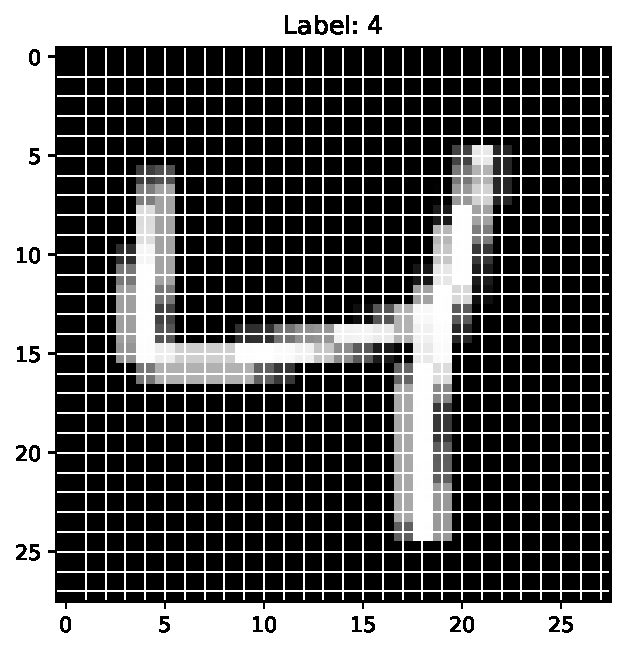
\includegraphics[scale=0.35]{../assets/accuracy-convention/figures/mnist.pdf}
			\end{notebookbox}
		  \end{figure}
		


	\end{frame}
		
	

\begin{frame}{Revision: What is Machine Learning}
	\begin{itemize}
	
	\item How would you program to recognise digits? Start with 4.
	
	\item \pause Maybe 4 can be thought of as: $\bm{|}$ + $\bm{\rule[0.5ex]{1em}{.95pt}}$ + $\bm{|}$ + another vertically down $\bm{|}$
	
	\item \pause The heights of each of the $\bm{|}$ need to be similar within tolerance
	
	\item \pause Each of the $\bm{|}$ can be slightly slanted. Similarly the horizontal line can be slanted.
	\item \pause There can be some cases of 4 where the first $\bm{|}$ is at 45 degrees
	\item \pause There can be some cases of 4 where the width of each stroke is different
	
\end{itemize}

\end{frame}	
  
 
\section{Machine Learning Fundamentals}

\begin{frame}{Traditional Programming vs Machine Learning}
\begin{center}
\begin{tikzpicture}[node distance=2cm]
  \node (D1) [startstop] {Data};
  \node (R1) [startstop, below of=D1] {Rules};
  \node (T1) [startstop, right of=D1, xshift=2cm, yshift=-1cm] {\makecell[l]{Traditional\\Programming}};
  \node (A1) [startstop, right of=T1, xshift=2cm] {Answers};
  \draw [arrow] (D1) -- (T1);
  \draw [arrow] (R1) -- (T1);
  \draw [arrow] (T1) -- (A1);
\end{tikzpicture}
\end{center}
\end{frame}


\begin{frame}{Traditional Programming}
\begin{tikzpicture}[node distance=2cm]
  \node (Data1) [startstop] {Data};
  \node (Rules1) [startstop, below of=Data1] {Rules};
  \node (Traditional) [startstop, right of=Data1, xshift=2cm, yshift=-1cm] {\makecell[l]{Traditional\\Programming}};
  \node (Answers1) [startstop, right of=Traditional, xshift=2cm] {Answers};
  \draw [arrow] (Data1) -- (Traditional);
  \draw [arrow] (Rules1) -- (Traditional);
  \draw [arrow] (Traditional) -- (Answers1);
\end{tikzpicture}
\end{frame}

\begin{frame}{Machine Learning}
\begin{tikzpicture}[node distance=2cm]
  \node (Data2) [startstop] {Data};
  \node (Answers2) [startstop, below of=Data2] {Answers};
  \node (ML) [startstop, right of=Data2, xshift=2cm, yshift=-1cm] {\makecell[l]{Machine \\Learning}};
  \node (Rules2) [startstop, right of=ML, xshift=2cm] {Rules};
  \draw [arrow] (Data2) -- (ML);
  \draw [arrow] (Answers2) -- (ML);
  \draw [arrow] (ML) -- (Rules2);
\end{tikzpicture}
\end{frame}

\begin{frame}{Revision: What is Machine Learning}
``A computer program is said to learn from
experience E with respect to some class of tasks T
and performance measure P if its performance at
tasks in T, as measured by P, improves with
experience E.'' - Tom Mitchell
\end{frame}

\section{First ML Example: Tomato Quality Prediction}

\begin{frame}{Pop Quiz \stepcounter{popquiz}\#\thepopquiz}
\begin{tcolorbox}[colback=blue!5!white,colframe=blue!75!black,title=Quick Question!]
In machine learning, which of the following is typically NOT a useful feature?
\begin{itemize}
	\item a) Color of a tomato for quality prediction
	\item b) Size of a house for price prediction  
	\item c) Sample ID number
	\item d) Age for medical diagnosis
\end{itemize}
\pause
\textbf{Answer:} c) Sample ID numbers are arbitrary identifiers, not meaningful features!
\end{tcolorbox}
\end{frame}

\begin{frame}{First ML Task: Grocery Store Tomato Quality Prediction}
Problem statement: You want to predict the quality of a tomato given its visual features.
\end{frame}

\begin{frame}{Dataset}
Imagine you have some past data on quality of tomatoes. What visual features do you think will be useful?

\begin{itemize}
	\item \pause Size
	\item \pause Colour
	\item \pause Texture
\end{itemize}
\end{frame}
  
\begin{frame}{Sample Dataset}
Here is our example dataset with tomato features: 

\begin{table}[]
	\begin{tabular}{|l|l|l|l||l|}
		\hline 
		\textbf{Sample} & \textbf{Colour} & \textbf{Size} & \textbf{Texture} & \textbf{Condition} \\ \hline 
		1      & Orange & Small & Smooth  & Good      \\
		2      & Red    & Small  & Rough  & Good \\
		3      & Orange & Medium & Smooth & Bad \\
		4      & Yellow & Large  & Smooth & Bad \\ \hline          
	\end{tabular}
\end{table}
\end{frame}

\begin{frame}{Useful Features}
Is the sample number a useful feature for predicting quality of a tomato?

\pause Answer: Usually no! Sample numbers are typically arbitrary identifiers and not meaningful features. Let us remove it.

\pause Let us modify our data table for now.

\begin{table}[]
	\begin{tabular}{|l|l|l||l|}
		\hline 
		\textbf{Colour} & \textbf{Size} & \textbf{Texture} & \textbf{Condition} \\ \hline 
		Orange & Small & Smooth  & Good      \\
		Red    & Small  & Rough  & Good \\
		Orange & Medium & Smooth & Bad \\
		Yellow & Large  & Smooth & Bad \\ \hline 

	\end{tabular}
\end{table}
\end{frame}

\begin{frame}{Training Set}

\begin{table}[]
	\begin{tabular}{|l|l|l||l|}
		\hline 
				\rowcolor{white}
		\textbf{Colour} & \textbf{Size} & \textbf{Texture} & \textbf{Condition} \\ \hline 
		Orange & Small & Smooth  & Good      \\
		Red    & Small  & Rough  & Good \\
		Orange & Medium & Smooth & Bad \\
		Yellow & Large  & Smooth & Bad \\ \hline 
		
	\end{tabular}
\end{table}

\pause The training set consists of two parts:
\begin{enumerate}
	\item \pause \color{Lavender}{Features (Input Variables)}
	\item \pause \color{Tan}{Output or Response Variable}
\end{enumerate}
\end{frame}

\begin{frame}{Training Set}
\vspace{-5pt}
\begin{table}[]
	\begin{tabular}{|l|l|l||l|}
		\hline 
		\rowcolor{white}
		\textbf{Colour} & \textbf{Size} & \textbf{Texture} & \textbf{Condition} \\ \hline 
		Orange & Small & Smooth  & Good      \\
		Red    & Small  & Rough  & Good \\
		Orange & Medium & Smooth & Bad \\
		Yellow & Large  & Smooth & Bad \\ \hline 
		
	\end{tabular}
\end{table}


\pause We call this matrix as $\cD$, containing:
\begin{enumerate}
	\item Feature matrix ($\mX \in \Real^{n \times d}$) containing data of $n$ samples each of which is $d$ dimensional.
	\item Output vector ($\vy \in \Real^n$) containing output variable for $n$ samples.
\end{enumerate}

\end{frame}

\begin{frame}{Data Matrix Details}
\begin{itemize}
	\item Feature matrix: $\mX = \begin{bmatrix} \vx_1\tp \\ \vx_2\tp \\ \vdots \\ \vx_n\tp \end{bmatrix}$ where $\vx_i \in \Real^d$
	\item \pause Example (after encoding): $\vx_1 = \begin{bmatrix}
	1 \\ 
	0 \\
	1 \\
	\end{bmatrix}$ (Orange=1, Small=0, Smooth=1)
	\item \pause Complete dataset: $\cD = \{(\vx_i\tp, y_i)\}_{i=1}^n$
\end{itemize}

\end{frame}


\begin{frame}{Prediction Task}
Estimate condition for unseen tomatoes (\#5, 6) based on data set. 

\begin{table}[]
	\begin{tabular}{|l|l|l||l|}
		\hline 
		
		\textbf{Colour} & \textbf{Size} & \textbf{Texture} & \textbf{Condition} \\ \hline 
		Orange & Small & Smooth  & Good      \\
		Red    & Small  & Rough  & Good \\
		Orange & Medium & Smooth & Bad \\
		Yellow & Large  & Smooth & Bad \\ \hline
		Red    & Large  & Rough  & ? \\
		Orange &  Large & Rough  & ? \\ \hline          
	\end{tabular}
\end{table}
\end{frame}

\begin{frame}{Testing Set}
\textcolor{YellowGreen}{Testing set} is similar to \textcolor{Peach}{training set}, but, does not contain labels for output variable. 

\begin{table}[]
	\begin{tabular}{|l|l|l||l|}
		\hline 
		\textbf{Colour} & \textbf{Size} & \textbf{Texture} & \textbf{Condition} \\ \hline 
		\rowcolor{Peach}
		Orange & Small & Smooth  & Good      \\
		\rowcolor{Peach}
		Red    & Small  & Rough  & Good \\
		\rowcolor{Peach}
		Orange & Medium & Smooth & Bad \\
		\rowcolor{Peach}
		Yellow & Large  & Smooth & Bad \\ \hline
				\rowcolor{YellowGreen}
		Red    & Large  & Rough  & ? \\
		\rowcolor{YellowGreen}
		Orange &  Large & Rough  & ? \\ \hline          
	\end{tabular}
\end{table}
\end{frame}



\begin{frame}{Prediction Task}
We hope to:
\begin{enumerate}
	\item \pause Learn $f$: 		$\text{Condition} = f(\text{colour, size, texture})$
	\item \pause From Training Dataset
	\item \pause To Predict the condition for the Testing set
\end{enumerate}


\begin{table}[]
	\begin{tabular}{|l|l|l||l|}
		\hline 
		
		\textbf{Colour} & \textbf{Size} & \textbf{Texture} & \textbf{Condition} \\ \hline 
		Orange & Small & Smooth  & Good      \\
		Red    & Small  & Rough  & Good \\
		Orange & Medium & Smooth & Bad \\
		Yellow & Large  & Smooth & Bad \\ \hline
		Red    & Large  & Rough  & ? \\
		Orange &  Large & Rough  & ? \\ \hline          
	\end{tabular}
\end{table}
\end{frame}

\begin{frame}{Generalisation}
\begin{itemize}
	\item Q: Is predicting on test set enough to say our model generalises? 
	\item \pause A: Ideally, no!
	\item \pause Ideally - we want to predict ``well'' on all possible inputs. But, can we test that?
	\item \pause No! Since, the test set is only a sample from all possible inputs.
\end{itemize}





\end{frame}

\begin{frame}{Generalisation}
\begin{figure}
	\centering
	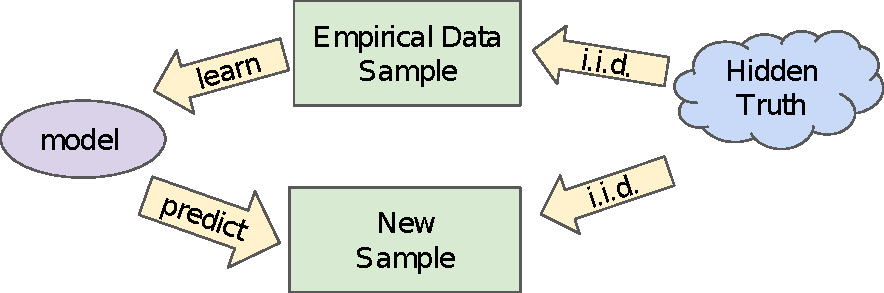
\includegraphics[width=0.8\textwidth]{../assets/accuracy-convention/diagrams/train-test.pdf}
	\caption{Image courtesy Google ML crash course}
	\label{fig:train-test}
\end{figure}

\pause Both the training set and the test set are samples drawn from the hidden true distribution (also sometimes called population)

\pause More discussion later once we study bias and variance
\end{frame}

\begin{frame}{Second ML Task: Predict energy consumption of campus}

Question: What factors does the campus energy consumption depend on?

Answer:\begin{itemize}
	\item \pause \# People (More people $\implies$ More Energy)
	\item \pause Temperature (Higher Temp. $\implies$ Higher Energy)

\pause \begin{table}[]
	\begin{tabular}{|l|l||l|}
		\hline 
		
		\textbf{\# People} & \textbf{Temp (C)} &  \textbf{Energy (kWh)} \\ \hline 
		
		4000 & 30 & 30 \\
		4200 & 30 & 32 \\
		4200 & 35 & 40 \\ \hline
		3000 & 20& ? \\
		1000 & 45 & ? \\ \hline          
	\end{tabular}
\end{table}	
\end{itemize}

\end{frame}





\section{Classification vs Regression}

\begin{frame}{Pop Quiz \stepcounter{popquiz}\#\thepopquiz}
\begin{tcolorbox}[colback=blue!5!white,colframe=blue!75!black,title=Quick Question!]
Which of these is a regression problem?
\begin{itemize}
	\item a) Predicting if an email is spam or not
	\item b) Classifying images as cat, dog, or bird
	\item c) Predicting house prices
	\item d) Determining if a tumor is malignant or benign
\end{itemize}
\pause
\textbf{Answer:} c) House prices are continuous values - that's regression!
\end{tcolorbox}
\end{frame}

\begin{frame}{Classification vs Regression}
\begin{itemize}
	\item Classification
	\begin{itemize}
		\item \pause Output variable is discrete
		\item \pause i.e.  $y_i \in \{1, 2, \ldots, k\}$ where $k$ is number of classes 
		\item \pause Examples - Predicting: 
		\begin{itemize}
			\item \pause Will I get a loan? (Yes, No)
			\item \pause What is the quality of fruit? (Good, Bad)
		\end{itemize}
	\end{itemize}
	\item \pause Regression
	\begin{itemize}
		\item \pause Output variable is continuous
		\item \pause i.e.  $y_i \in \Real$ 
		\item \pause Examples - Predicting: 
		\begin{itemize}
			\item \pause How much energy will campus consume? 
			\item \pause How much rainfall will fall?
		\end{itemize}
	\end{itemize}
\end{itemize}

\end{frame}



%\captionsetup[subtable]{labelformat=empty}
%
%\begin{frame}{Metrics for Classification}
%\begin{table}[!htb]
%	\caption{}
%	\begin{subtable}{.5\linewidth}
%		\centering
%		\caption{Prediction ($\yhat$)}
%		\begin{tabular}{ |c| } \hline 
%			
%			Good \\
%			Good \\
%			Good \\
%			Good \\
%			Bad  \\ \hline 
%			
%		\end{tabular}
%	\end{subtable}%
%	\begin{subtable}{.5\linewidth}
%		\centering
%		\caption{Ground Truth ($\vy$)}
%		\begin{tabular}{ |c| } 
%			\hline 
%			Good \\
%			Good \\
%			Bad \\
%			Bad  \\
%			Bad \\ \hline 
%		\end{tabular} \\
%	\end{subtable} 
%\end{table}
%
%\begin{align*}
%\text{Accuracy} &= \frac{||y = \hat{y}||}{||y||} \end{align*}
%\end{frame}

%\begin{frame}{Metrics for Classification}
%\begin{table}[!htb]
%	\caption{}
%	\begin{subtable}{.5\linewidth}
%		\centering
%		\caption{Prediction ($\yhat$)}
%		\begin{tabular}{ |c| } \hline 
%			
%			\rowcolor{Green}Good \\
%			\rowcolor{Green}Good \\
%			\rowcolor{Red}Good \\
%			\rowcolor{Red}Good \\
%			\rowcolor{Green}Bad  \\ \hline 
%			
%		\end{tabular}
%	\end{subtable}%
%	\begin{subtable}{.5\linewidth}
%		\centering
%		\caption{Ground Truth ($\vy$)}
%		\begin{tabular}{ |c| } 
%			\hline 
%			Good \\
%			Good \\
%			Bad \\
%			Bad  \\
%			Bad \\ \hline 
%		\end{tabular} \\
%	\end{subtable} 
%\end{table}
%
%\begin{align*}
%\text{Accuracy} &= \frac{||y = \hat{y}||}{||y||} \\
%&= \frac{3}{5} = 0.6
%\end{align*}
%\end{frame}
%
%%\begin{frame}
%%\setlength{\tabcolsep}{12pt}
%%\begin{tabular}{ cc }   % top level tables, with 2 rows
%%	Ground Truth ($\vy$) & Prediction ($\yhat$) \\  
%%	% bottom left of the top level table: table 1 
%%	\begin{tabular}{ |c| } 
%%		
%%		Good \\
%%		Good \\
%%		Good \\
%%		Good \\
%%		Bad  \\
%%		
%%	\end{tabular} &  % starting bottom right of the top level table
%%	% table 2
%%	\begin{tabular}{ |c| } 
%%		Good \\
%%		Good \\
%%		Bad \\
%%		Bad  \\
%%		Bad \\
%%	\end{tabular} \\
%%\end{tabular}
%%\end{frame}
%%
%%\begin{frame}{Metrics for Classification}
%%
%%
%%
%%$
%%Prediction (\hat{y}) = \begin{bmatrix}
%%	Good \\
%%	Good \\
%%	Good \\
%%	Good \\
%%	Bad  \\
%%\end{bmatrix} ~~~~Ground Truth (y) = \begin{bmatrix}
%%Good \\
%%Good \\
%%Bad \\
%%Bad  \\
%%Bad \\
%%\end{bmatrix}$ 
%%\vspace{30pt}
%%
%%\begin{itemize}
%%	\item Ground Truth: From the actual training set 
%%	\item Prediction: Made by the model
%%\end{itemize}
%%
%%\end{frame}
%%
%%\begin{frame}{Metrics for Classification}
%%%\DoTikzmark{num-3}{-}3 & 0 & {4}\DoTikzmark{num4}
%%$
%%Prediction (\hat{y}) = \begin{bmatrix}
%%Good \\
%%Good \\
%%Good \\
%%Good \\
%%Bad  \\
%%\end{bmatrix} ~~~~Ground Truth (y) = \begin{bmatrix}
%%Good \\
%%Good \\
%%Bad \\
%%Bad  \\
%%Bad \\
%%\end{bmatrix}$ 
%%
%%
%%\vspace{30pt}
%
%
%
%%\end{frame}


\section{Classification Metrics}

\begin{frame}{Metrics for Classification}



$$\bordermatrix{&\text{Prediction}\;(\hat{y})\cr
                &\text{Good}\cr
                &\text{Good}\cr
                &\text{Good}\cr
                &\text{Good}\cr
                &\text{Bad}}
                \qquad \qquad
   \bordermatrix{&\text{Ground Truth}\;(\vy)\cr
                &\text{Good}\cr
                &\text{Good}\cr
                &\text{Bad}\cr
                &\text{Bad}\cr
                &\text{Bad}}
$$

\vspace{1cm}

\begin{tabular}{ll}
Ground Truth: & From the actual training set \\ 
Prediction: & Made by the model \\ 
\end{tabular}

\end{frame}

\begin{frame}{Accuracy}
$$
\bordermatrix{&\text{Prediction}\;(\hat{y})\cr
               \checkmark&\text{Good}\cr
               \checkmark&\text{Good}\cr
                &\text{Good}\cr
                &\text{Good}\cr
               \checkmark&\text{Bad}}
\qquad \qquad
\bordermatrix{&\text{Ground Truth}\;(\vy)\cr
                &\text{Good}\cr
                &\text{Good}\cr
                &\text{Bad}\cr
                &\text{Bad}\cr
                &\text{Bad}}
$$

\pause \begin{align*}
\text{Accuracy} &= \frac{|\{i : y_i = \hat{y}_i\}|}{n} \\ 
&= \frac{3}{5} = 0.6
\end{align*}

\end{frame}

\begin{frame}{Mathematical Notation: Set Cardinality and Indicator Functions}
\begin{itemize}
	\item \pause \textbf{Set cardinality notation:} $|\{i : y_i = \hat{y}_i\}|$ 
	\begin{itemize}
		\item Reads as: ``Number of indices $i$ such that $y_i = \hat{y}_i$''
		\item Counts how many samples satisfy the condition
	\end{itemize}
	
	\item \pause \textbf{Alternative: Indicator function notation}
	\begin{align*}
	\text{Accuracy} &= \frac{\sum_{i=1}^n \mathbf{1}[y_i = \hat{y}_i]}{n}
	\end{align*}
	where $\mathbf{1}[\text{condition}] = \begin{cases} 1 & \text{if condition is true} \\ 0 & \text{if condition is false} \end{cases}$
	
	\item \pause Both notations are mathematically equivalent and commonly used in ML literature
\end{itemize}
\end{frame}

\begin{frame}{Types of Data: Imbalanced Classes}
\[
  \begin{array}{@{} c @{}}
    \begin{array}{@{} r @{}}
      \text{1 sample}~\{\hspace{\nulldelimiterspace} \\
      \text{100 samples}~\left\{\begin{array}{@{}c@{}}\null\\\null\\\null\\\null\end{array}\right.
    \end{array}
    \left (
      \begin{array}{ *{1}{c} }
        \text{Bad}  \\
        \text{Good}  \\
        \text{Good}  \\
        \ldots  \\
        \text{Good}  \\
      \end{array}
    \right ) \\
    \mathstrut
  \end{array}
  \quad \quad \quad
  \text{Imbalanced Classes}
\]

\pause

Cases for this:
\begin{itemize}%[<+->]
\item Cancer Screening
\item Planet Detection
\end{itemize}

\end{frame}

\begin{frame}{Accuracy Metrics: Precision}
$$
\bordermatrix{&\text{Prediction}\;(\hat{y})\cr
               \rightarrow\checkmark&\text{Good}\cr
               \rightarrow\checkmark&\text{Good}\cr
                \rightarrow&\text{Good}\cr
                \rightarrow&\text{Good}\cr
               &\text{Bad}}
\qquad \qquad
\bordermatrix{&\text{Ground Truth}\;(\vy)\cr
                &\text{Good}\cr
                &\text{Good}\cr
                &\text{Bad}\cr
                &\text{Bad}\cr
                &\text{Good}}
$$

\begin{align*}
\pause \text{Precision} &= \frac{|\{i : y_i = \hat{y}_i = \text{Good}\}|}{|\{i : \hat{y}_i = \text{Good}\}|} = \frac{2}{4} = 0.5
\end{align*}

``the fraction of relevant instances among the retrieved instances'', i.e. ``out of the number of times we predict \text{Good}, how many times is the condition actually \text{Good}''

\end{frame}

\begin{frame}{Accuracy Metrics: Recall}
$$
\bordermatrix{&\text{Prediction}\;(\hat{y})\cr
               \rightarrow\checkmark&\text{Good}\cr
               \rightarrow\checkmark&\text{Good}\cr
                &\text{Good}\cr
                &\text{Good}\cr
               \rightarrow&\text{Bad}}
\qquad \qquad
\bordermatrix{&\text{Ground Truth}\;(\vy)\cr
                &\text{Good}\cr
                &\text{Good}\cr
                &\text{Bad}\cr
                &\text{Bad}\cr
                &\text{Good}}
$$

\begin{align*}
\text{Recall} &= \frac{|\{i : y_i = \hat{y}_i = \text{Good}\}|}{|\{i : y_i = \text{Good}\}|} = \frac{2}{3} = 0.67
\end{align*}

``the fraction of the total amount of relevant instances that were actually retrieved''

\end{frame}

\begin{frame}{Pop Quiz \stepcounter{popquiz}\#\thepopquiz}
\begin{tcolorbox}[colback=blue!5!white,colframe=blue!75!black,title=Quick Question!]
In a dataset of 1000 samples where only 10 are positive cases, what's the accuracy of a classifier that always predicts ``negative''?
\begin{itemize}
	\item a) 1\%
	\item b) 50\% 
	\item c) 90\%
	\item d) 99\%
\end{itemize}
\pause
\textbf{Answer:} d) 99\% - but this classifier is useless! This shows why accuracy can be misleading.
\end{tcolorbox}
\end{frame}

\begin{frame}{Types of Data: Imbalanced Classes}
Given predictions of whether a tissue is cancerous or not ($n = 100$).
$$
\bordermatrix{&\text{Prediction}\;(\hat{y})\cr
               \rightarrow&\text{Yes}\cr
               &\text{No}\cr
                &\text{No}\cr
                &\ldots\cr
               &\text{No}}
\qquad \qquad
\bordermatrix{&\text{Ground Truth}\;(\vy)\cr
                &\text{No}\cr
                &\text{No}\cr
                &\ldots\cr
                &\text{No}\cr
                \rightarrow&\text{Yes}}
            $$

\pause 
\begin{align*}
\text{Accuracy} = \frac{98}{100} = 0.98 \qquad \qquad \qquad
\text{Recall} &= \frac{0}{1} = 0 \\
\text{Precision} &= \frac{0}{1} = 0
\end{align*}


\end{frame}

\begin{frame}{Accuracy Metrics: Confusion Matrix}
\begin{center}


\begin{tabular}{@{}cc cc@{}}
	\multicolumn{1}{c}{} &\multicolumn{1}{c}{} &\multicolumn{2}{c}{Ground Truth} \\ 
	\cmidrule(lr){3-4}
	\multicolumn{1}{c}{} & 
	\multicolumn{1}{c}{} & 
	\multicolumn{1}{c}{Yes} & 
	\multicolumn{1}{c}{No} \\ 
	\cline{2-4}
	\multirow[c]{2}{*}{\rotatebox[origin=tr]{90}{Predicted}}
	& Yes  & 0 & 1   \\[1.5ex]
	& No  & 1   & 98 \\ 
	\cline{2-4}
\end{tabular}

\pause 
\vspace{60pt}
\begin{tabular}{@{}cc cc@{}}
	\multicolumn{1}{c}{} &\multicolumn{1}{c}{} &\multicolumn{2}{c}{Ground Truth} \\ 
	\cmidrule(lr){3-4}
	\multicolumn{1}{c}{} & 
	\multicolumn{1}{c}{} & 
	\multicolumn{1}{c}{Yes} & 
	\multicolumn{1}{c}{No} \\ 
	\cline{2-4}
	\multirow[c]{2}{*}{\rotatebox[origin=tr]{90}{Predicted}}
	& Yes  & True Positive & False Positive   \\[1.5ex]
	& No  & False Negative   & True Negative \\ 
	\cline{2-4}
\end{tabular}
\end{center}
\end{frame}

\begin{frame}{Accuracy Metric: Confusion Matrix}
\begin{center}
	\begin{tabular}{@{}cc cc@{}}
		\multicolumn{1}{c}{} &\multicolumn{1}{c}{} &\multicolumn{2}{c}{Ground Truth} \\ 
		\cmidrule(lr){3-4}
		\multicolumn{1}{c}{} & 
		\multicolumn{1}{c}{} & 
		\multicolumn{1}{c}{Yes} & 
		\multicolumn{1}{c}{No} \\ 
		\cline{2-4}
		\multirow[c]{2}{*}{\rotatebox[origin=tr]{90}{Predicted}}
		
		& Yes  & \cellcolor{blue!25}True Positive & \cellcolor{blue!25}False Positive   \\[1.5ex]
		& No  & False Negative   & True Negative \\ 
		\cline{2-4}
	\end{tabular}\\
	
	\vspace{30pt}
	Precision = $\frac{\text{TP}}{\text{TP} + \text{FP}}$
\end{center}
\end{frame}

\begin{frame}{Accuracy Metric: Confusion Matrix}
\begin{center}
\begin{tabular}{@{}cc cc@{}}
	\multicolumn{1}{c}{} &\multicolumn{1}{c}{} &\multicolumn{2}{c}{Ground Truth} \\ 
	\cmidrule(lr){3-4}
	\multicolumn{1}{c}{} & 
	\multicolumn{1}{c}{} & 
	\multicolumn{1}{c}{Yes} & 
	\multicolumn{1}{c}{No} \\ 
	\cline{2-4}
	\multirow[c]{2}{*}{\rotatebox[origin=tr]{90}{Predicted}}
	
	& Yes  & \cellcolor{blue!60}True Positive & \cellcolor{blue!25}False Positive   \\[1.5ex]
	& No  & False Negative   & True Negative \\ 
	\cline{2-4}
\end{tabular}\\

\vspace{30pt}
Precision = $\frac{\text{TP}}{\text{TP} + \text{FP}}$
\end{center}
\end{frame}

\begin{frame}{Accuracy Metric: Confusion Matrix}
\begin{center}
	\begin{tabular}{@{}cc cc@{}}
		\multicolumn{1}{c}{} &\multicolumn{1}{c}{} &\multicolumn{2}{c}{Ground Truth} \\ 
		\cmidrule(lr){3-4}
		\multicolumn{1}{c}{} & 
		\multicolumn{1}{c}{} & 
		\multicolumn{1}{c}{Yes} & 
		\multicolumn{1}{c}{No} \\ 
		\cline{2-4}
		\multirow[c]{2}{*}{\rotatebox[origin=tr]{90}{Predicted}}
		
		& Yes  & \cellcolor{blue!25}True Positive &False Positive   \\[1.5ex]
		& No  &  \cellcolor{blue!25}False Negative   & True Negative \\ 
		\cline{2-4}
	\end{tabular}\\
	
	\vspace{30pt}
	Recall = $\frac{\text{TP}}{\text{TP} + \text{FN}}$
\end{center}
\end{frame}

\begin{frame}{Accuracy Metric: Confusion Matrix}
\begin{center}
	\begin{tabular}{@{}cc cc@{}}
		\multicolumn{1}{c}{} &\multicolumn{1}{c}{} &\multicolumn{2}{c}{Ground Truth} \\ 
		\cmidrule(lr){3-4}
		\multicolumn{1}{c}{} & 
		\multicolumn{1}{c}{} & 
		\multicolumn{1}{c}{Yes} & 
		\multicolumn{1}{c}{No} \\ 
		\cline{2-4}
		\multirow[c]{2}{*}{\rotatebox[origin=tr]{90}{Predicted}}
		
		& Yes  & \cellcolor{blue!50}True Positive &False Positive   \\[1.5ex]
		& No  &  \cellcolor{blue!25}False Negative   & True Negative \\ 
		\cline{2-4}
	\end{tabular}\\
	
	\vspace{30pt}
	Recall = $\frac{\text{TP}}{\text{TP} + \text{FN}}$
\end{center}
\end{frame}


%\begin{frame}{Accuracy Metrics: Confusion Matrix}
%For the same data
%\pause $$
%\bordermatrix{&\text{G.T. Positive}&\text{G.T. Negative}\cr
%               \text{Pred Positive}&0&1\cr
%               \text{Pred Negative}&1&98}
%$$
%\pause $$
%\bordermatrix{&\text{G.T. Positive}&\text{G.T. Negative}\cr
%               \text{Pred Positive}&\text{True Positive}&\text{False Positive}\cr
%               \text{Pred Negative}&\text{True Negative}&\text{False Negative}}
%$$
%
%
%\pause \begin{align*}
%\text{Recall} = \frac{\text{T.P}}{\text{T.P + F.P}} \qquad \qquad 
%\text{Precision} = \frac{\text{T.P}}{\text{T.P + F.N}}
%\end{align*}
%\end{frame}

\begin{frame}{Accuracy Metrics: F-Score}

\begin{center}
	\begin{tabular}{@{}cc cc@{}}
		\multicolumn{1}{c}{} &\multicolumn{1}{c}{} &\multicolumn{2}{c}{Ground Truth} \\ 
		\cmidrule(lr){3-4}
		\multicolumn{1}{c}{} & 
		\multicolumn{1}{c}{} & 
		\multicolumn{1}{c}{Yes} & 
		\multicolumn{1}{c}{No} \\ 
		\cline{2-4}
		\multirow[c]{2}{*}{\rotatebox[origin=tr]{90}{Predicted}}
		
		& Yes  & True Positive &False Positive   \\[1.5ex]
		& No  &  False Negative   & True Negative \\ 
		\cline{2-4}
	\end{tabular}\\
	
	\vspace{30pt}
	\(\mathrm{F}-\) Score \(=\frac{2 \times \text { Precision } \times \text { Recall }}{\text { Precision }+\text { Recall }}\)

\end{center}
\end{frame}


\begin{frame}{Accuracy Metrics: Matthew's Correlation Coefficient}
\begin{center}
	\begin{tabular}{@{}cc cc@{}}
		\multicolumn{1}{c}{} &\multicolumn{1}{c}{} &\multicolumn{2}{c}{Ground Truth} \\ 
		\cmidrule(lr){3-4}
		\multicolumn{1}{c}{} & 
		\multicolumn{1}{c}{} & 
		\multicolumn{1}{c}{Yes} & 
		\multicolumn{1}{c}{No} \\ 
		\cline{2-4}
		\multirow[c]{2}{*}{\rotatebox[origin=tr]{90}{Predicted}}
		
		& Yes  & True Positive &False Positive   \\[1.5ex]
		& No  &  False Negative   & True Negative \\ 
		\cline{2-4}
	\end{tabular}\\

\vspace{30pt}
Matthew's correlation coefficient =
\(\frac{\mathrm{TP} \times \mathrm{TN}-\mathrm{FP} \times \mathrm{FN}}{\sqrt{(\mathrm{TP}+\mathrm{FP})(\mathrm{TP}+\mathrm{FN})(\mathrm{TN}+\mathrm{FP})(\mathrm{TN}+\mathrm{FN})}}\)
\end{center}
\end{frame}



\begin{frame}{Accuracy Metrics: Example}
For the data given below, calculate: 
$$
\bordermatrix{&\text{G.T. Positive}&\text{G.T. Negative}\cr
               \text{Pred Positive}&90&4\cr
               \text{Pred Negative}&1&1}
$$

Precision = ?  \\
Recall = ?\\
F-Score = ?\\
Matthew's Coeff. = ?\\
\end{frame}

\begin{frame}{Accuracy Metrics: Answer}
For the same data
$$
\bordermatrix{&\text{G.T. Positive}&\text{G.T. Negative}\cr
               \text{Pred Positive}&90&4\cr
               \text{Pred Negative}&1&1}
$$

Precision = $\frac{90}{94}$ \\
Recall = $\frac{90}{91}$ \\
F-Score = 0.9524 \\
Matthew's Coeff. = 0.14
\end{frame}


\begin{frame}{Confusion Matrix for multi-class classification}
	\begin{figure}[htp]
		\centering
		\begin{notebookbox}{https://nipunbatra.github.io/ml-teaching/notebooks/confusion-mnist.html}
		  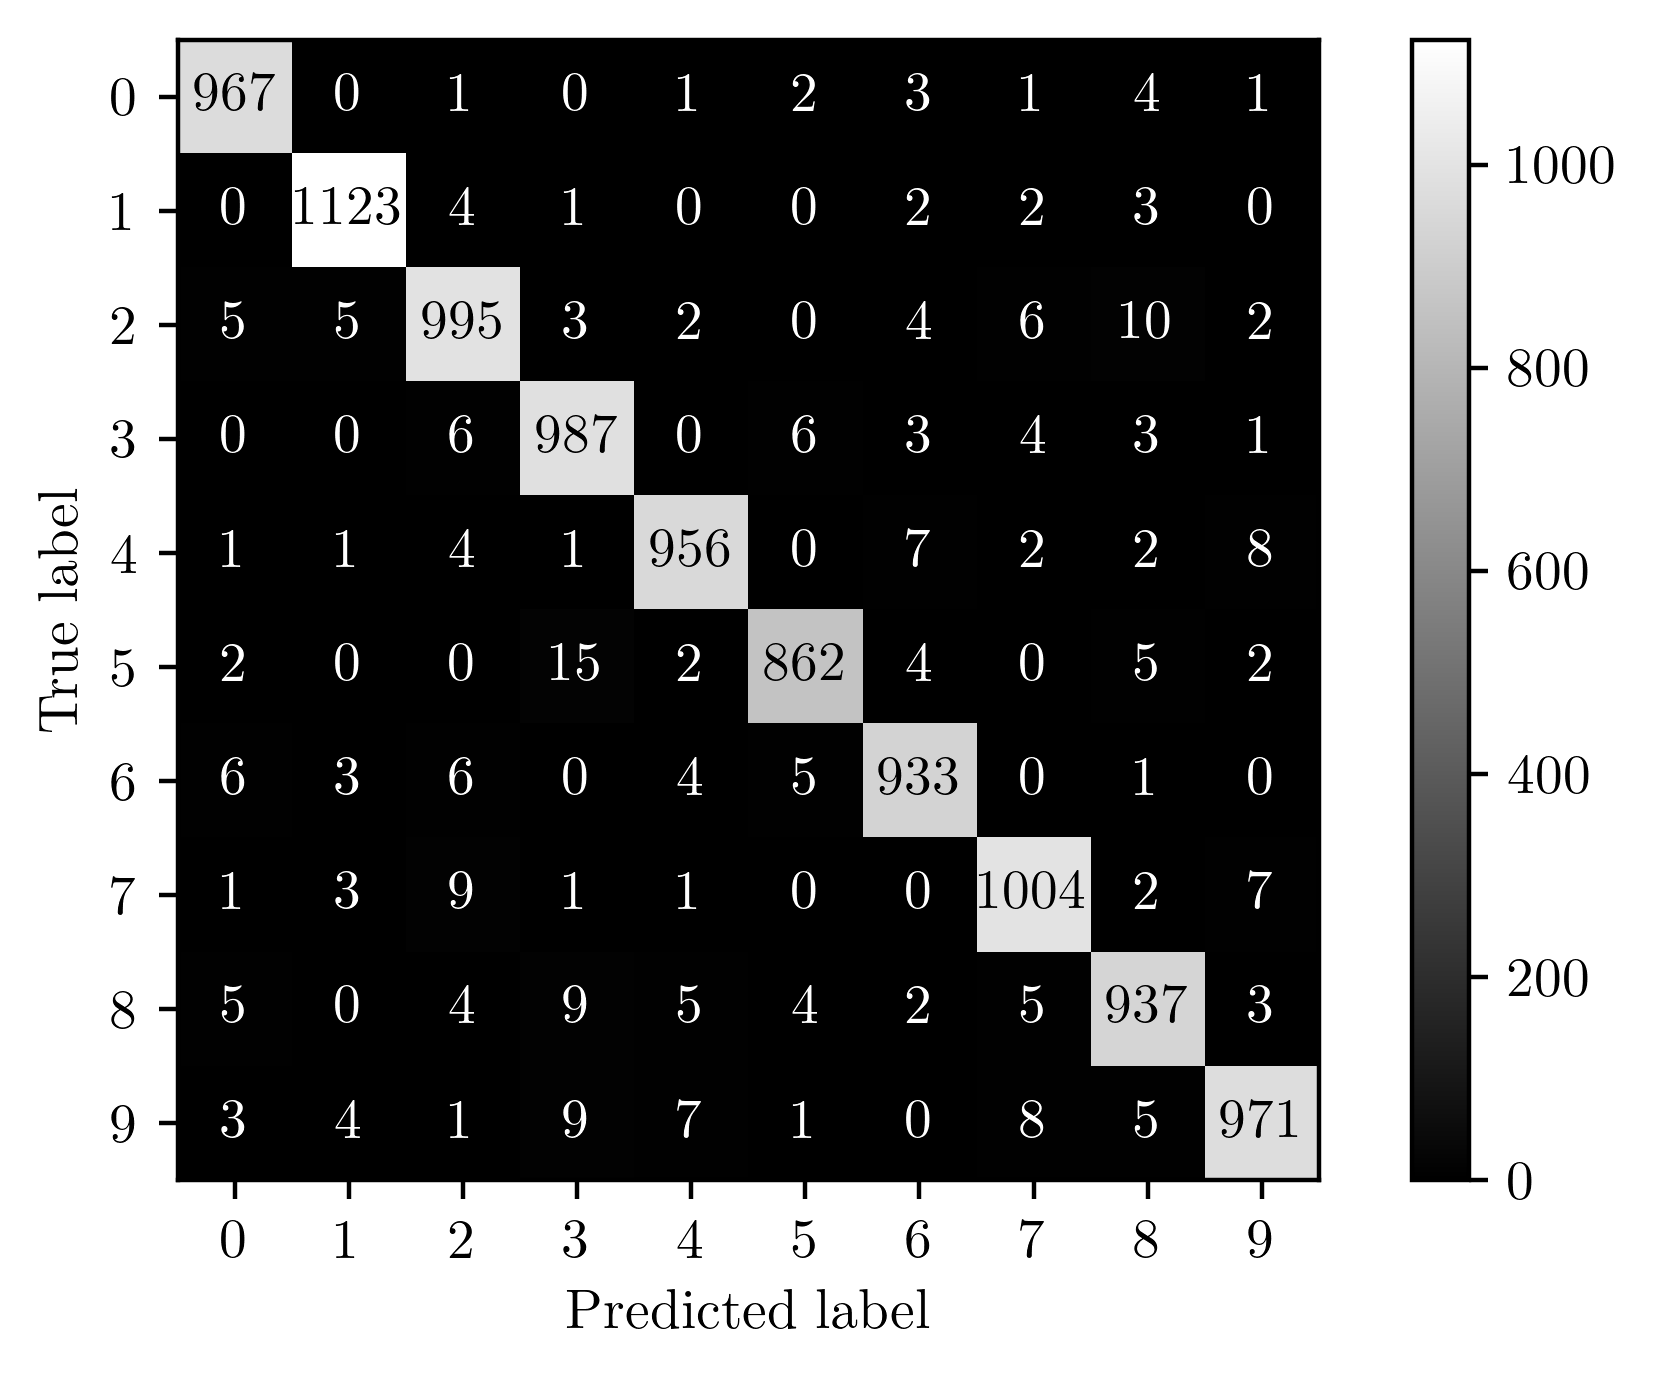
\includegraphics[scale=0.5]{../assets/accuracy-convention/figures/mnist-cm.png}
		\end{notebookbox}
	  \end{figure}
	
\end{frame}



\section{Regression Metrics}

\begin{frame}{Pop Quiz \stepcounter{popquiz}\#\thepopquiz}
\begin{tcolorbox}[colback=blue!5!white,colframe=blue!75!black,title=Quick Question!]
Why might Mean Absolute Error (MAE) be preferred over Mean Squared Error (MSE)?
\begin{itemize}
	\item a) MAE is always smaller
	\item b) MAE is less sensitive to outliers
	\item c) MAE is easier to compute
	\item d) MAE works only for classification
\end{itemize}
\pause
\textbf{Answer:} b) MAE is less sensitive to outliers since it doesn't square the errors!
\end{tcolorbox}
\end{frame}

\begin{frame}{Metrics for Regression: MSE \& MAE}
$$
\bordermatrix{&\text{Prediction}\;(\hat{y})\cr
               &10\cr
               &20\cr
                &30\cr
                &40\cr
               &50}
\qquad \qquad
\bordermatrix{&\text{Ground Truth}\;(\vy)\cr
               &20\cr
               &30\cr
                &40\cr
                &50\cr
               &60}
$$

\begin{align*}
\text{\textcolor{red}{Mean} \textcolor{green}{Squared} \textcolor{Tan}{Error} (MSE)} &=  \frac{\mathcolor{red}{\sum_{i=1}^{n}}(\mathcolor{Tan}{\hat{y}_i-y_i)}^{\mathcolor{green}2}}{\mathcolor{red}{n}} \\ 
\text{Root Mean Square Error (RMSE)} &=  \sqrt{\text{MSE}}
\end{align*}

\end{frame}

\begin{frame}{Accuracy Metrics: MAE \& ME}
$$
\bordermatrix{&\text{Prediction}\;(\hat{y})\cr
               &10\cr
               &20\cr
                &30\cr
                &40\cr
               &50}
\qquad \qquad
\bordermatrix{&\text{Ground Truth}\cr
               &20\cr
               &30\cr
                &40\cr
                &50\cr
               &60}
$$

\begin{align*}
\text{\textcolor{red}{Mean} \textcolor{green}{Absolute} \textcolor{Tan}{Error} (MAE)} &=  \frac{\mathcolor{red}{\sum_{i=1}^{n}}\mathcolor{green}|\mathcolor{Tan}{\hat{y}_i-y_i\mathcolor{green}|}}{\mathcolor{red}{n}} \\ 
\text{Mean Error} &=  \frac{\sum_{i=1}^{n}(\hat{y}_i-y_i)}{n}
\end{align*}
\pause Is there any downside with using mean error?\\
\pause Errors can get cancelled out

\end{frame}

\section{Data Visualization and Baselines}

\begin{frame}{The Importance of Plotting}
    \begin{figure}[htp]
      \centering
      \begin{notebookbox}{https://nipunbatra.github.io/ml-teaching/notebooks/anscombe.html}
        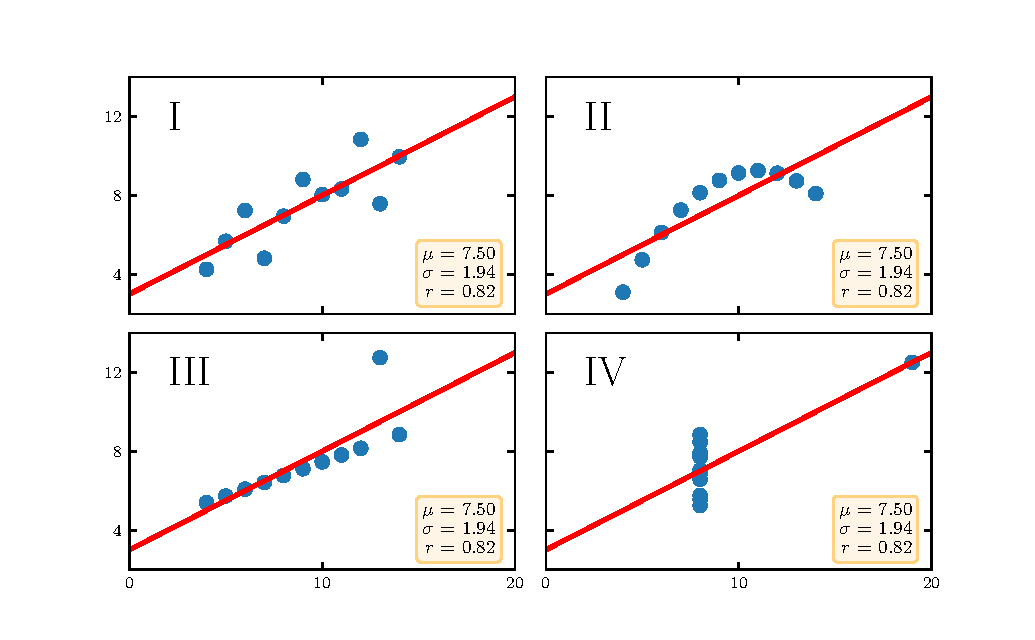
\includegraphics[width=\linewidth]{../assets/accuracy-convention/figures/anscombe.pdf}
      \end{notebookbox}
      \caption{Anscombe’s Quartet}
    \end{figure}
  \end{frame}

  \begin{frame}{Dummy Baselines}
	\begin{notebookbox}{https://nipunbatra.github.io/ml-teaching/notebooks/dummy-baselines.html}
	  \end{notebookbox}
\end{frame}

\begin{frame}{The Importance of Plotting}
\begin{tabular}{|c|c|c|}
\hline 
Property & Value & Across datasets \\ 
\hline 
mean(X) & 9 & exact \\ 
mean(Y) & 7.5 & up to 3 decimal places \\ 
Linear regression line & 	y = 3.00 + 0.500x & up to 2 decimal places \\ 
\hline 
\end{tabular} 


\end{frame}

\section{Summary and Key Takeaways}

\begin{frame}{Pop Quiz \stepcounter{popquiz}\#\thepopquiz}
\begin{tcolorbox}[colback=blue!5!white,colframe=blue!75!black,title=Final Challenge!]
For imbalanced datasets, which metrics should you prioritize over accuracy?
\begin{itemize}
	\item a) Only precision
	\item b) Only recall
	\item c) Precision, recall, and F1-score
	\item d) Only confusion matrix
\end{itemize}
\pause
\textbf{Answer:} c) Precision, recall, and F1-score give a more complete picture!
\end{tcolorbox}
\end{frame}

\begin{frame}{Key Takeaways}
\begin{itemize}
	\item \textbf{ML vs Traditional Programming:} ML learns rules from data, traditional programming uses predefined rules
	\item \textbf{Features matter:} Choose meaningful features, avoid arbitrary identifiers
	\item \textbf{Classification vs Regression:} Discrete outputs vs continuous outputs
	\item \textbf{Accuracy isn't everything:} For imbalanced data, use precision, recall, F1-score
	\item \textbf{Visualization is crucial:} Always plot your data (Anscombe's Quartet lesson)
	\item \textbf{Use baselines:} Simple baseline models help validate your approach
\end{itemize}
\end{frame}

\begin{frame}{Summary: Evaluation Metrics}
\begin{center}
\begin{tabular}{|l|l|l|}
\hline
\textbf{Task} & \textbf{Common Metrics} & \textbf{When to Use} \\
\hline
\textbf{Classification} & Accuracy, Precision, Recall, F1 & Balanced/Imbalanced data \\
 & Confusion Matrix & Multi-class problems \\
\hline
\textbf{Regression} & MSE, RMSE, MAE & Continuous predictions \\
 & Mean Error & Check for bias \\
\hline
\end{tabular}
\end{center}

\vspace{1cm}
\textbf{Remember:} Choose metrics based on your problem's characteristics and business requirements!
\end{frame}

\end{document}
